\vfill

\begin{center}
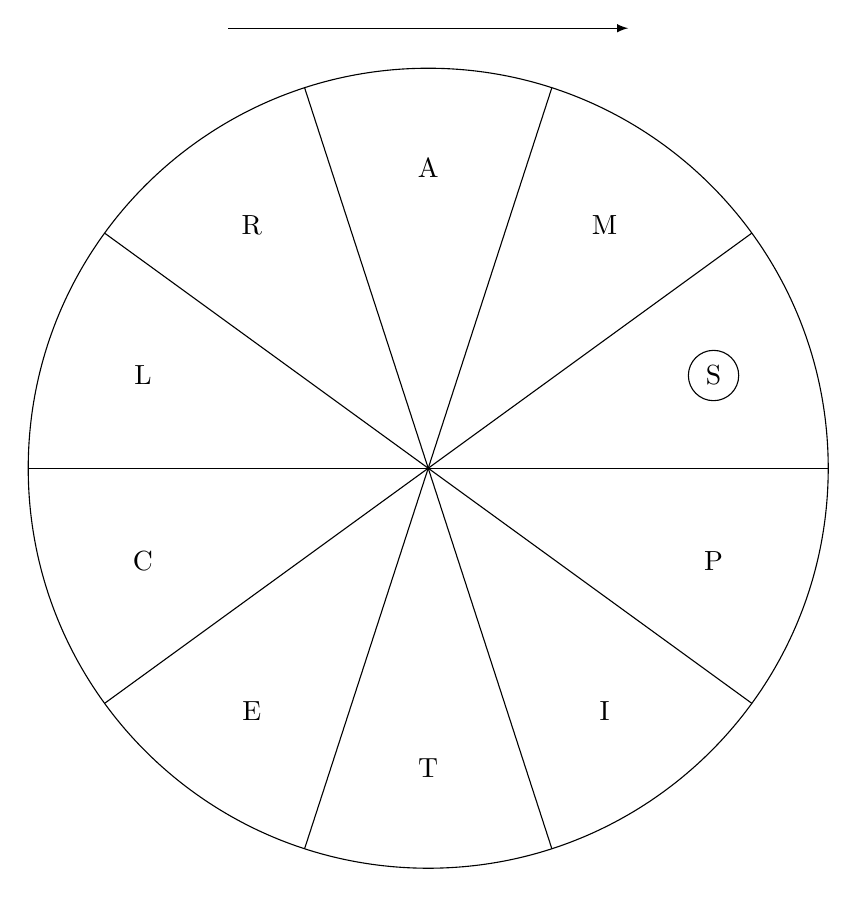
\begin{tikzpicture}[x=1in,y=1in]
\draw (0,0) circle (2);
\draw (0:2) -- (180:2);
\draw (36:2) -- (-144:2);
\draw (72:2) -- (-108:2);
\draw (108:2) -- (-72:2);
\draw (144:2) -- (-36:2);
\node[draw,circle] at (18:1.5) {S};
\node at (54:1.5) {M};
\node at (90:1.5) {A};
\node at (126:1.5) {R};
\node at (162:1.5) {L};
\node at (-162:1.5) {C};
\node at (-126:1.5) {E};
\node at (-90:1.5) {T};
\node at (-54:1.5) {I};
\node at (-18:1.5) {P};
\draw[-latex] (-1,2.2) -- (1,2.2);
\end{tikzpicture}
\end{center}

\vfill
%{
%  \LARGE
%  \normalfont\wedn
%It seems that the legendary rulers of the Skolem people
%were each associated with a compass direction.
%Fascinating!
%
%\renewcommand{\labelitemi}{}
%\begin{itemize}
%\item Oystein Apo Skolem (N)
%\item Engstrom Apo Ore (NNE) % 7 O
%\item Throralf Apo Thue (NE)
%\item Shanok Apo Ore (ENE)
%\item Trowa Apo Ore (E)
%\item Mawort Apo Ore (ESE) % 5 R
%\item Berkov Apo Kel (SE)
%\item Knutten Apo Kel (SSE)
%\item Erbach Apo Kel (S)
%\item Guabis Apo Kel (SSW) % 5 I
%\item Zabala Apo Dheub (SW)
%\item Renfrow Apo Dheub (WSW) % 6 O
%\item Frakov Apo Dheub (W)
%\item Gangolli Apo Dheub (WNW) % 3 N
%\item Ramkunar Apo Lewo (NW)
%\item Skraba Apo Lewo (NNW)
%%\item Govc Apo Preis 1686 - 1675 BCE
%\end{itemize}
%}
